%%%%%%%%%%%%%%%%%%%%%%%%%%%%%%%%%%%%%%%%%%%%%%%%%%%%%%%%%%%%%%%%%%%%%%%%
% Plantilla TFG/TFM
% Escuela Politécnica Superior de la Universidad de Alicante
% Realizado por: Jose Manuel Requena Plens
% Contacto: info@jmrplens.com / Telegram:@jmrplens
%%%%%%%%%%%%%%%%%%%%%%%%%%%%%%%%%%%%%%%%%%%%%%%%%%%%%%%%%%%%%%%%%%%%%%%%

\chapter{Tecnologías}
\label{3.Tecnologias}

    Una vez definido el problema a tratar, los objetivos generales y específios del proyecto, la solución propuesta y los requisitos a implementar hay que analizar las herramientas y tecnologías a utilizar. Para esto habrá que plantearse diferentes modelos y tecnologías disponibles para el desarrollo y optar por aquellos que aporten estabilidad y buen rendimiento.

    \section{Modelos}

        En primer lugar analizaremos los modelos utilizados durante la realización del proyecto.

        \subsection {Algoritmos Genéticos}
            Un \textit{Algoritmo Genético} \cite{GA}, es un modelo que imita la evolución de las especies en el ámbito de la biología, con el objetivo de encontrar una solución potencialmente óptima a un problema. El planteamiento de estos modelos consiste en evaluar los individuos pertenecientes a la población de la generación correspondiente para tomar el subconjunto de aquellas soluciones que mejor calidad ofrezcan mediante una función heurística denominada \textit{función fitness} que aproxima soluciones ideales a un problema.\\

            Hay que remarcar que las funciones heurísticas son funciones aproximadas a una solución ideal del problema, debido a que todas las posibles combinaciones de los parámetros a optimizar genera un espacio de búsqueda exponencial (problema NP-hard), es necesario crear una aproximación mediante la función heurística para acotar éste espacio.\\

            Para comprender el funcionamiento de los algoritmos genéticos es necesario analizar cada una de las fases que lo constituyen:
            
            \begin{enumerate}
                \item Inicialización de la Población:

                        En primer lugar es necesario generar los \textit{n} individuos de la población aleatoriamente. Cada uno de estos individuos está formado por el conjunto de parámetros que son objeto de optimización \ref{InitialPopulation}.

                        \begin{figure}[h]
                            \centering
                            \includesvg[inkscapelatex=false]{archivos/3.Tecnologias/GA/InitialPopulation}
                            \caption{Inicialización de la población. Cada individuo está constituido por n parámetros del XGBoost a optimizar.}
                            \label{InitialPopulation}
                        \end{figure}

                \item Evaluación de Población:

                        Es la primera fase del proceso iterativo del algoritmo genético y, en él, cada uno de los individuos pertenecientes a la población son evaluados mediante la función \textit{fitness}.

                \item Selección de Padres:

                        Una vez evaluados los individuos de la población, se procede a seleccionar aquellos que mejor valor han obtenido para crear nuevas soluciones a partir de éstos padres. Existen distintas técnicas de selección, como por ejemplo escoger aquellos \textit{n} mejores padres de la población o técnicas basadas en métodos probabilísticos, para que aquellos individuos que menos puntuación logren, tengan alguna probabilidad de ser elegidos para la generación de nuevas soluciones. Este tipo de técnicas se utilizan para aumentar la diversidad en la pobĺación y evitar caer en soluciones acotadas a mínimos locales del problema. Se puede ver el proceso de cómo son seleccionados los padres en función de su \textit{fitness} en la figura \ref{FitnessFunction}.

                        \begin{figure}[h]
                            \centering
                            \includesvg[inkscapelatex=false]{archivos/3.Tecnologias/GA/FitnessFunction}
                            \caption{Selección de padres candidatos.}
                            \label{FitnessFunction}
                        \end{figure}

                \item Cruce:

                        Una vez seleccionados los padres es necesario que intercambien información entre ellos para dar lugar a nuevos individuos, este proceso de herencia de información es posible realizarlo aplicando distintas filosofías; seleccionar un punto o posición de cruce a lo largo del vector de los padres y combinar ambos padres, o escoger aleatoriamente las posiciones de los parámetros de ambos padres y combinarlos para dar lugar a la solución generada figura [\ref{ParentsMatingMutationImage}].

                        \begin{figure}[h]
                            \centering
                            \includesvg[inkscapelatex=false]{archivos/3.Tecnologias/GA/ParentsMatingMutation}
                            \caption{Mutación de hijos.}
                            \label{ParentsMatingMutationImage}
                        \end{figure}

                \item Mutación:

                        Cuando los padres seleccionados son combinados para dar lugar a los candidatos de la nueva generación, es importante aplicar un proceso de mutación entre éstos debido a la necesidad de generar diversidad en la población. Si se combina la misma información entre generaciones se corre el riesgo de converger prematuramente a un mínimo local del espacio de búsqueda. Por este motivo se introduce el concepto de mutación, que consiste en aplicar una modificación aleatoria sobre alguno de los parámetros de los individuos generados para poder ampliar el espacio de soluciones. 
            \end{enumerate}

            Cada una de las fases enumeradas anteriormente se repite de forma iterativa entre generaciones hasta que se cumpla alguna condición de parada.


            A continuación enumeraremos los parámetros con los que configurar un algoritmo genético. Dependiendo del tipo de algoritmo utilizado es posible encontrar distintos parámetros con los que inicializar el algoritmo, sin embargo estos son los más extendidos:


            \begin{itemize}


                \item Probabilidad de cruce: probabilidad con la que dos padres intercambian su información entre sí para dar lugar a un nuevo individuo hijo.

                \item Probabilidad de mutación: indica la probabilidad con la que cada hiperparámetro puede variar su valor.

            \end{itemize}


        \subsection {XGBoost}

            
            \textit{Extreme Gradient Boosting Algortihm} (\textit{XGBoost}) es una libería open-source que implementa algoritmos \textit{ML Ensembles de tipo Boosting}. Se trata unos algoritmos muy utilizado en los últimos años, logrando un rendimiento diez veces mayor a otras soluciones populares en una misma máquina y llegando a las primeras posiciones en numerosos retos propuestos en \textit{Kaggle} \cite{XGBoostTutorial}.\\

            XGBoost se basa en los modelos \textit{Ensemble Boosting} de los algoritmos de \textit{ML}, de ahí su nombre \textit{Gradient Boosting}. La técnica \textit{Boosting} se basa en construir un modelo robusto (\textit{strong learner}) combinando una serie de modelos débiles (\textit{weak learners}) \cite{NvidiaXGBoost}.\\


            Concretamente \textit{XGBoost} implementa \textit{Gradient Boosting Decision Trees (GBDT)}, que es un algoritmo similar a los \textit{Random Forest}, y es utilizado tanto para clasificación como para regresión.\\

            La diferencia principal entre los algoritmos \textit{Random Forest} y \textit{XGBoost} radica en el hecho de que los primeras utilizan algoritmos \textit{Ensembles} tipo \textit{Bagging} y construyen un modelo final predictivo mediante en el que la salida será la combinación de las predicciones de cada uno de los modelos individuales. En el caso de los modelos \textit{Ensembles Boosting} (\textit{XGBoost}) se combinan secuencialmente de forma que su objetivo es minimizar el error producido los árboles generales utilizando para ello el método de descenso por gradiente.\\


            En la figura [\ref{XGBoostFlowImage}] se puede observar cómo se van construyendo los árboles clasificadores y cómo cada árbol minimiza el residuo producido por el árbol anterior.\\


            \begin{figure}[h]
                \centering
                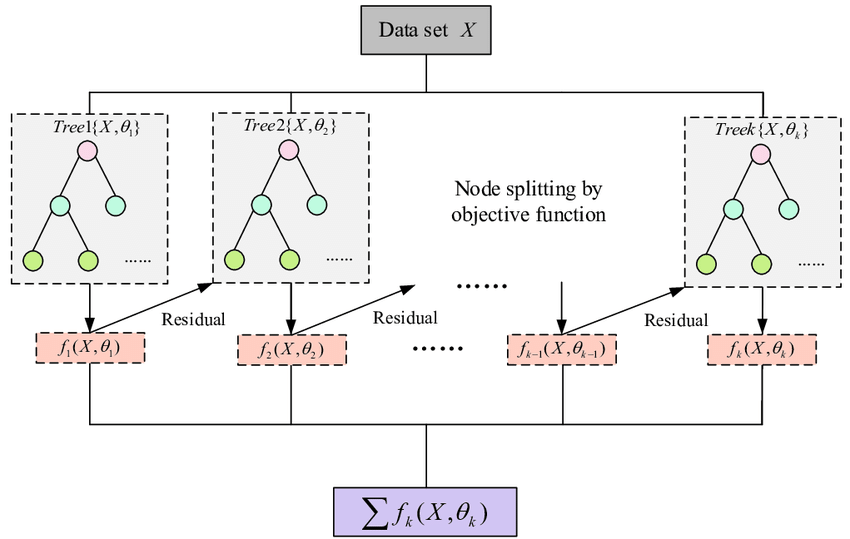
\includegraphics[width=10cm]{archivos/3.Tecnologias/XGBoost/XGBoostFlowImage}
                \caption{Proceso de optimización de XGBoost.}
                \label{XGBoostFlowImage}
             \end{figure}

            
            Además, \textit{XGBoost} aplica técnicas de regularización en su función de pérdida, de tal forma que reduce la influencia individual de cada árbol generado y de sus hojas para poder dar lugar a posteriores árboles que consigan mejorar el modelo, evitando de esta manera el sobreajuste u \textit{overfitting}.


        \subsection {Gaussian Naive Bayes}

        \textcolor{red}{El clasificador probabilístico \glsentryfull{nb} es un modelo que se basa en el \textit{Teorema de Bayes}, este clasificador asume ciertas suposiciones de independencia sobre los predictores para realizar las clasificaciones. Se asume que la presencia o ausencia de cualquier predictor no está condicionada por la inclusión o exclusión de cualquier otro en el conjunto de datos, es decir, cualquier característica de las observaciones es independiente del resto. Asumiendo esta independencia entre los predictores la complejidad computacional del modelo se reduce considerablemente, haciendo de este modelo uno de los más eficientes en aprendizaje estadístico.}

        \textcolor{red}{Para utilizar Naive Bayes con valores reales se asume la distribución Gaussiana de las características, a esta adaptación se le denomina como \glsentryfull{gnb}. Este enfoque es más simple que el anterior ya que únicamente es necesario calcular la media y la desviación típica de las variables de entrada para resumir dichas distribuciones, que se utilizarán para calcular la probabilidad de pertenencia a una clase en función de estas distribuciones normales gracias a la media y a la desviación típica de cada variable.}

        \textcolor{red}{El primer paso será calcular la denominada probabilidad a priori, que es la probabilidad de que una nueva muestra pertenezca a alguna de las clases del conjunto de entrenamiento, este cálculo serviŕá para determinar la predicción final de las observaciones.}

        \textcolor{red}{Posteriormente se calculará, para cada una de las variables de la muestra, la probabilidad de pertenecer a cada clase del conjunto de entrenamiento en función del grado de pertenencia a la distribución Gaussiana correspondiente a la variable. Después se aplicará esta multiplicación de probabilidades a la probabilidad a priori inicial definida a dicha clase.}

        \textcolor{red}{En la siguiente fórmula se define la probabilidad de pertenencia a una clase $c$ del conjunto $Y$ en base a la característica $X$.}

        \begin{center}
            $ P(X|Y = c) = \frac{1}{\sqrt{2 \pi \sigma^{2}_{c}}} e^{\frac{- (x - \mu_c)^2}{2 \sigma^{2}_{c}}}$
        \end{center}

        \textcolor{red}{Donde $\sigma$ es la varianza y $\mu$ es la media de la variable $X$ perteneciente a la clase $c$ del conjunto de clases posibles $Y$.}

        \subsection {SVC}


             \textcolor{red}{Los \glsentryfull{svc}, también denominados como \textit{Soft Margin Classifier}, son modelos orientados a clasificación múltiple \cite{SVM}. Se basan en proyectar los datos de entrada en un espacio multidimensional buscando la separabilidad las estas muestras en este espacio determinando hiperplanos.}\\

            \textcolor{red}{Los \glsentryshort{svc} construyen estos hiperplanos en base a la máxima separabilidad de las clases utilizando únicamente aquellas observaciones que se encuentren en la fronteras que maximizan la distancia en el plano entre las clases. La ventaja de esta técnica es que es necesario un conjunto muy pequeño de muestras de entrenamiento para sostener los hiperplanos que forman las fronteras de decisión, estos puntos se denominan \textit{vectores de soporte}.}\\

            \textcolor{red}{La distancia entre los vectores de soporte y el hiperplano definido es denominado \textit{margen}, y es en este punto donde entra en juego la flexibilidad de los \glsentryshort{svc}. Estos modelos aplican el denominado \textit{margen blando}, que se basa en permitir que ciertas observaciones se encuentren en un lado erróneo del margen o incluso del hiperplano, haciendo que el modelo sea más robusto permitiendo mayor generalización a costa de clasificar erróneamente alguna de las observaciones mediante un parámetro de tolerancia $C$. A un mayor valor de $C$ se permite que un mayor número de muestras violen el margen \citep{ISLR2}}.\\


            \textcolor{red}{En la figura \cite{SVCExampleImage} se muestra un ejemplo aplicado de \glsentryshort{svc}, donde se observan los hiperplanos definidos que maximiza la separabilidad de ambas clases y los vectores de soporte definidos en función de distintos valores de tolerancia $C$.}

            \begin{figure}[h]
                \centering
                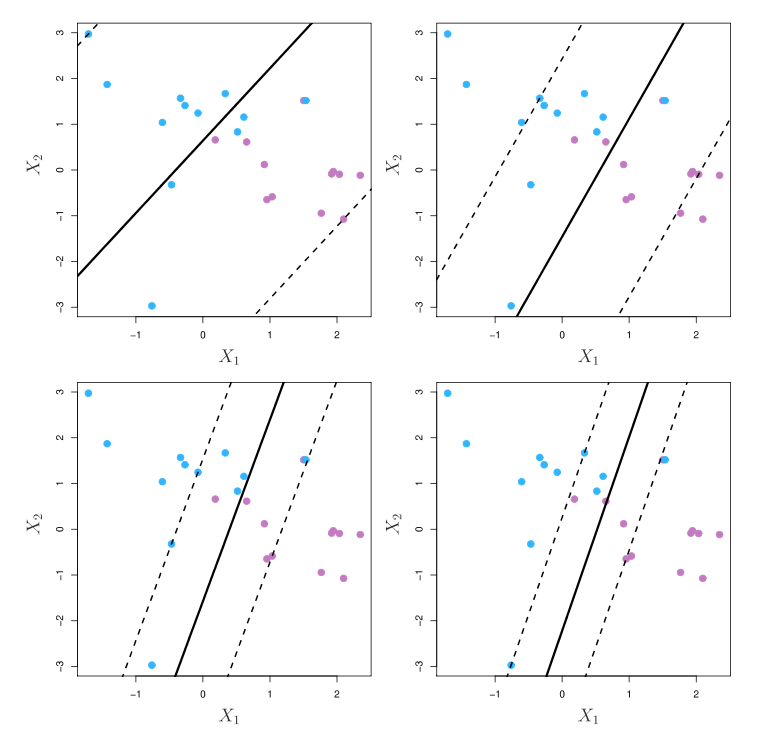
\includegraphics[width=10cm]{archivos/3.Tecnologias/SVC/SVCExample}
                \caption{ISLR2. Ejemplo de SVC con distintos valores de C.}
                \label{SVCExampleImage}
             \end{figure}

        \subsection {Redes Neuronales}

            Las Redes Neuronales \cite{NNReview} son modelos que emulan comportamiento del cerebro a la hora de procesar la información, entrenándose sobre un conjunto de datos de entrenamiento para identificar patrones entre ellos.\\

            A modo de comprensión, se muestra la arquitectura de una \textit{NN}, donde se pueden observar las conexiones entre cada capa de la red y sus salidas en la figura \ref{NNImage}. Existe una capa de entrada inicial que corresponde a cada una de las características del ejemplo de entrada (en el caso de imágenes se trata de cada uno de los píxeles). Cada una de las características de la capa de entrada se conecta con cada una de las neuronas de la primera capa oculta \textit{hidden layer} a través de conexiones denominadas pesos (\textit{weights}) que son los que serán aprendidos en la red con el objetivo de encontrar patrones entre las características mediante el método de \textit{Descenso por Gradiente} o \textit{Gradient Descent (GD)}.\\


            Esta metodología se aplica para cada una de las \textit{hidden layers} presentes en la arquitectura hasta la última capa, llegando hasta la última función \textit{SoftMax} que dictará la clase predicha en base a la salida de la capa final, u \textit{output layer}.\\

            \begin{figure}[h]
                \centering
                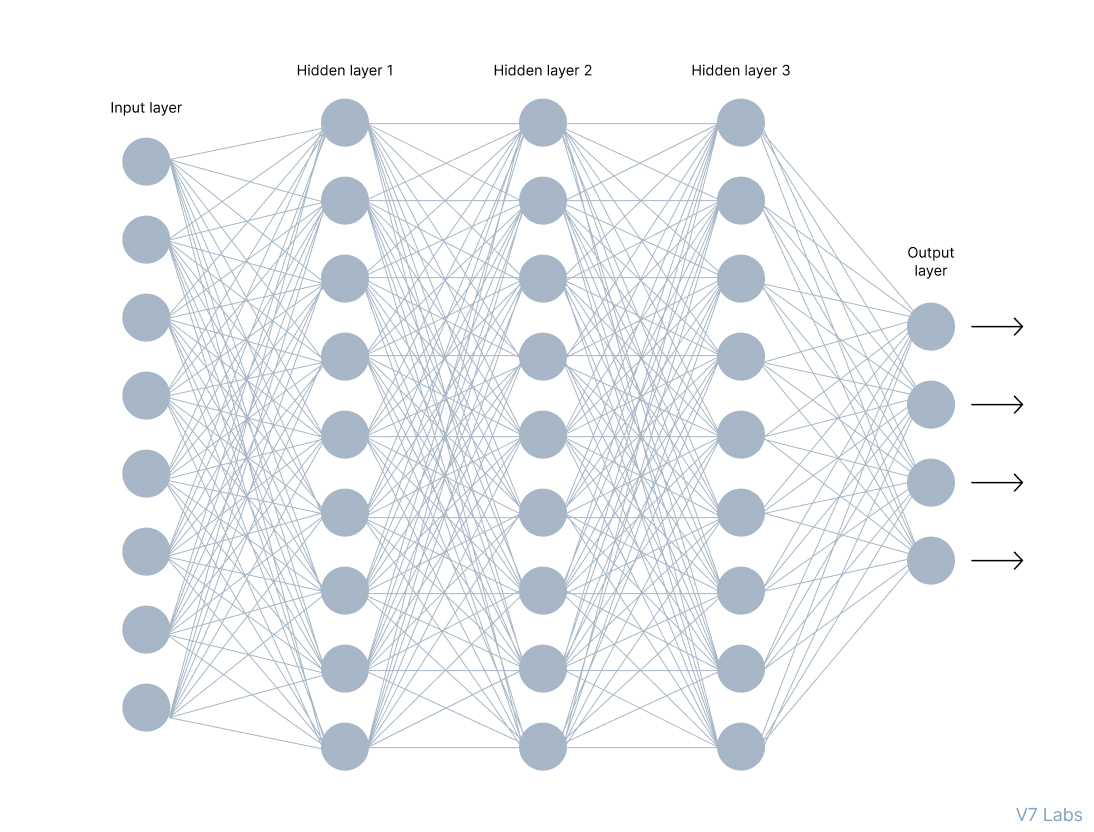
\includegraphics[width=10cm]{archivos/3.Tecnologias/RedesNeuronales/NNImage}
                \caption{https://www.v7labs.com/blog/neural-networks-activation-functions. Arquitectura de una Red Neuronal.}
                \label{NNImage}
             \end{figure}



            Existen una serie de conceptos comunes a todas las \textit{NN} que es conveniente nombrar para su comprensión:


            \begin{itemize}

                \item Función de activación: las funciones de activación son las encargadas de decidir si una neurona es activada o no en función de la entrada a esta función. Esta función suele situarse en la salida de cada capa de la red para decidir si una determinada neurona de la siguiente capa se activa o no.

                    Existen distintos enfoques en lo que respecta a las funciones de activación, como la función logística, tangente hiperbólica y \textit{softmax} entre otras.


                \item Entropía: la entropía sobre una varible aleatoria $X$ es el grado de incertidumbre producido en base a los posibles valores que puede tomar como respuesta. Se calcula en base a la siguiente fórmula:

                    \begin{center}
                        $H(X) = -\sum_{i = 1}^n p(x_i) \log_2 p(x_i)$
                    \end{center}

                    Donde $x_i$ es cada uno de los posibles valores que puede tomar la variable como respuesta y $p(x_i)$ es la probabilidad de obtener dicho valor. 


                \item Softmax: se trata de la generalización en forma multidimensional de la función logística o \textit{logistic function}. \textit{Softmax} es una función que permite la transformación de un vector de números reales a una distribución de probabilidad. Esta función se suele aplicar como capa de activación en el último nivel en las \textit{NN}, representando la probabilidad de que la salida de la red pertenezca a cada una de las $K$ clases posibles en el modelo \cite{Softmax}. 

                    Esto es necesario debido a que normalmente los componentes de la salida de la última capa de una red neuronal (\textit{logits}) son el resultado de la predicción en forma de números reales no normalizados, por lo tanto pueden ser mayores que $1$ e incluso negativos. La función permite calcular la distribución de probabilidad en base a estos \textit{logits} y calcular la probabilidad de pertenencia de la muestra a cada una de las $K$ clases que componen el modelo mediante la siguiente fórmula:


                    \begin{center}
                        $\sigma(z_i) = \frac{e^{z_{i}}}{\sum_{j=1}^K e^{z_{j}}} \ \ \ for\ i=1,2,\dots,K$
                    \end{center}


                    Esta función es continua y diferenciable, por lo que es posible aplicar el método \textit{GD} para actualizar los valores de los pesos de la red neuronal en las capas anteriores gracias a estas propiedades que permiten la derivabilidad de la función.


                \item Cross-Entropy: el objetivo de cross-entropy es minimizar la función de pérdida (\textit{log loss}) comparando la probabilidad de la clase predicha con respecto a su valor verdadero. Al aplicar una penalización logarítmica, las probabilidades de las clases que más disten respecto a su valor verdadero se verán más acentuadas \cite{Cross-Entropy}.

                    \begin{center}
                        $L_{CE} = -\sum_{i = 1}^n y_i \log_2(p_i)$
                    \end{center}

                    Donde $n$ es el número de clases a predecir, el valor $y_i$ es la etiqueta de la clase verdadera, y $p_i$ es la probabilidad de que la muestra actual pertenezca a la clase $i$.

                    \begin{figure}[h]
                        \centering
                        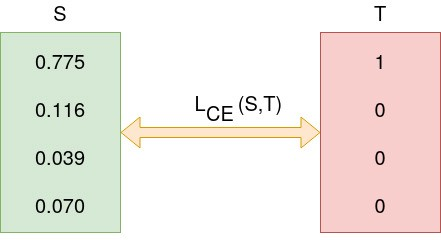
\includegraphics[width=7cm]{archivos/3.Tecnologias/RedesNeuronales/CrossEntropy}
                        \caption{https://towardsdatascience.com/cross-entropy-loss-function-f38c4ec8643e Cross-Entropy entre la función Softmax (izquierda) y el valor de la clase verdadera (derecha).}
                        \label{CrossEntropyImage}
                     \end{figure}

                \item Back Propagation: en el proceso de entrenamiento de la \textit{NN} es necesario actualizar los pesos de las capas ocultas con el objetivo de minimizar la cross-entropy total del modelo. Para minimizar este valor se utiliza un algoritmo de optimización que maximiza el valor de una función \textit{GD}.

                    Gracias a las propiedades de la función \textit{Softmax} es posible utilizar descenso por gradiente para calcular la derivada de la función de pérdida respecto de cada uno de los pesos de las capas intermedias de la red y actualizar cada uno de ellos con el objetivo de minimizar la función de pérdida.

                \item Learning Rate: la \textit{tasa de aprendizaje}, o \textit{learning rate} define el tamaño de paso que se aplicará a a la hora de optimizar los pesos de la red. El valor del \textit{learning rate} se comprende en el intervalo $[0,1]$, de tal forma que a menor valor de la tasa de aprendizaje menor será el cambio que se produce en los pesos de las neuronas del modelo, el caso contrario ocurre cuando adopta un valor alto.\\



                    Este parámetro no es sencillo de especificar, el \textit{learning rate} es un regularizador que con valores altos permite que la red no caiga en \textit{overfitting}, caso que ocurriría si el valor fuera demasiado pequeño y la minimización de la función de pérdida cayese en un mínimo local debido a aprender demasiado de los datos de entrenamiento. Si el valor es muy alto los pesos de los parámetros de la red variarán excesivamente impidiendo la convergencia en un mínimo de la función.\\

                    Esta disyuntiva ha sido ampliamente estudiada en los últimos tiempos, acerca de cuál es el valor ideal del \textit{learning rate} en las \textit{NN} \cite{LearningRate}, aunque comunmente se configura con el valor $0.1$.



                \item Batch Normalization: el proceso de entrenamiento de una red neuronal puede ser costoso, ya que existen una gran cantidad de parámetros para cada capa que son optimizados durante el proceso de entrenamiento. Esto hace que este proceso sea demasiado sensible a los parámetros inicializados en el inicio del entrenamiento de la red, como es el ejemplo de establecer una tasa de aprendizaje \textit{learning rate} muy baja para poder converger. Esto hace que el entrenamiento sea muy lento, por lo que es necesario normalizar las entradas para cada mini-batch (subconjuntos de datos de entrenamiento con el que se entrena la red en cada época.\\


                    El método \textit{Batch Normalization} \cite{BatchNormalization} normaliza los datos de tal forma que permite utilizar tasas de aprendizaje mayores además de actuar como regularizador, reduciendo así el número de capas \textit{Dropout} que pudieran existir en la arquitectura.

            \end{itemize}

            \subsubsection{Convolucionales}

                A contiuación definiremos los parámetros específicos aplicados a las \glsentryfull{cnn2d}:

                \begin{itemize}

                    \item Kernels:

                        Son las estructuras que se encargan de realizar la convolución. Los kernels son matrices de pesos unidimensionales ($1 \times n$) o bidimensionales ($n \times m$) dependiendo del tipo de convolución que se esté aplicando (Convolución 1-D o Convolución 2-D), y se encargan de inferir patrones en la matriz de entrada gracias a la actualización de sus pesos. En función de la profundidad de la capa, los kernels podrán encontrar patrones más simples o más complejos debido a que la entrada a cada capa es una convolución (aplicación del filtro) de las capas anteriores.

                        Un kernel realiza el producto escalar de sus pesos con respecto a las posiciones de la matriz de entrada (imagen o \textit{feature map}) que colisionen en ese momento con el kernel, generando un nuevo \textit{feature map} de menor dimensión, a menos que se utilice la técnica de \textit{Padding} \cite{Kernels}.
                         
                    \item Filtros:

                        Un filtro no es más que una agrupación de kernels, siempre tendrán una dimensión mayor que la definida para el kernel. Por ejemplo, si disponemos de un kernel unidimensional ($1 \times n$), el filtro contendrá $k$ kernels de ($1 \times n$) en la capa convolucional definida \cite{FiltersFeatureMaps}

                    \item Strides:

                        Son los saltos producidos por un kernel en cada etapa de la convolución, dependiendo si la convolución es dimensional o bidimensional, el stride constará de una dimensión ($i$), es decir, los pasos hacia la derecha en la imagen, o de dos dimensiones ($i, j$), los pasos hacia la derecha y hacia abajo en la imagen.

                        \begin{figure}[h]
                            \centering
                            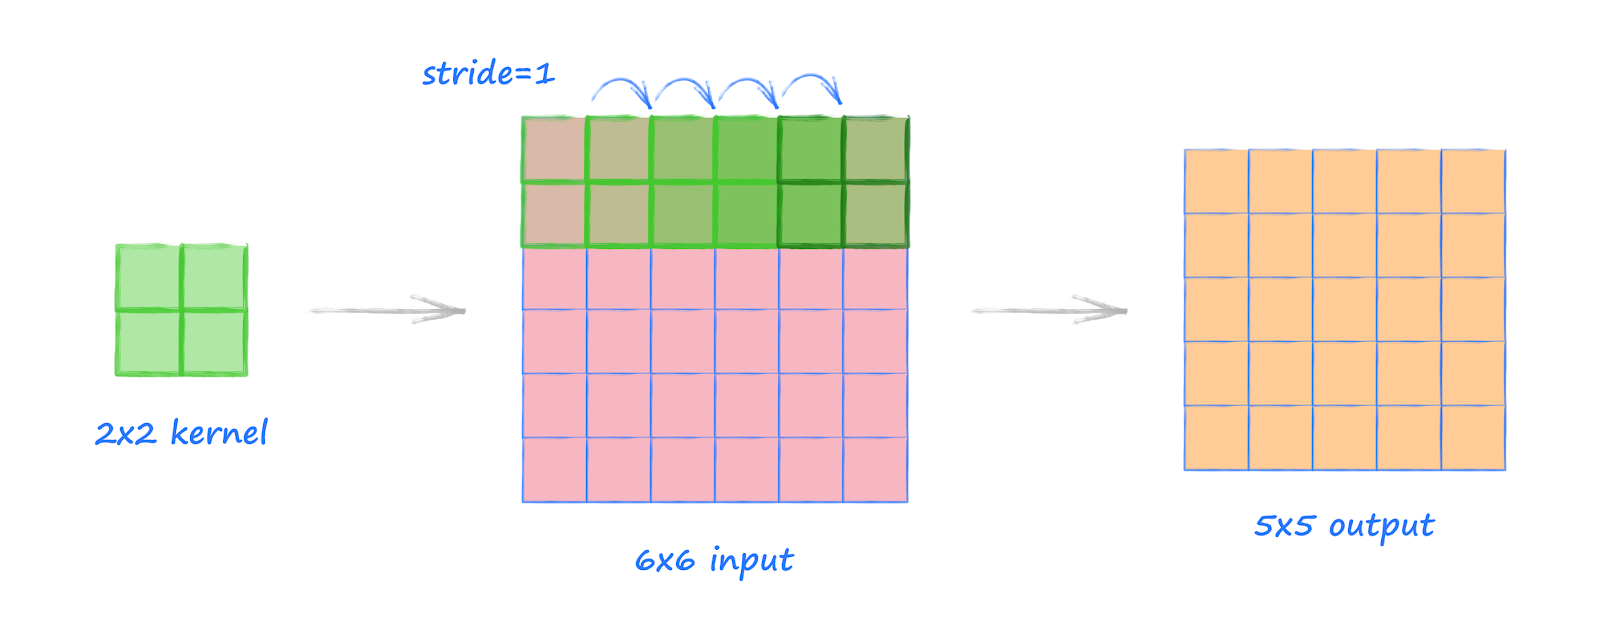
\includegraphics[width=10cm]{archivos/3.Tecnologias/RedesNeuronales/Stride}
                            \caption{http://makeyourownneuralnetwork.blogspot.com/2020/02/calculating-output-size-of-convolutions.html}
                            \label{StrideImage}
                         \end{figure}

                    \item Padding:

                        El padding es un método utilizado para incrementar la dimensionalidad de la entrada de la capa debido el desvanecimiento de los valores posicionados en zonas comprometedoras una vez aplicada la convolución.\\

                        El \textit{padding} es el proceso de generar celdas artificiales inicializadas con valor \textit{0} que permiten que el filtro convolucional sea aplicado en su totalidad en la posición de estas zonas comprometedoras, manteniendo la información de los límites de la imagen. De otra forma ĺos valores de estos extremos se desvanecerían a medida se incrementa la profundidad de la red (número de capas) con respecto al resto de valores de la matriz.\\

                        \begin{figure}[h]
                            \centering
                            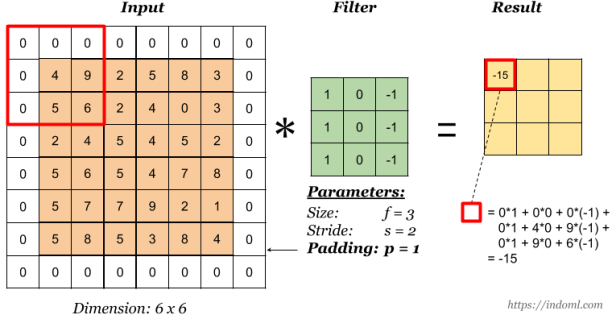
\includegraphics[width=10cm]{archivos/3.Tecnologias/RedesNeuronales/CNN/padding}
                            \caption{https://indoml.com/2018/03/07/student-notes-convolutional-neural-networks-cnn-introduction/}
                            \label{PaddingImage}
                         \end{figure}


                    \item Función de activación:


                        En el caso de las redes neuronales convolucionales, la función de activación se aplica a cada casilla proyectada por cada kernel sobre la matriz de entrada, de tal forma que cambia el valor a $0$ sobre aquellos valores que resulten negativos de la convolución.\\

                        En la figura \ref{CNNRELUImage} se puede apreciar cómo se aplica la función de activación \textit{ReLU} para cada casilla de la proyección de un \textit{kernel} bidimensinoal sobre una \textit{red convolucional de dos dimensiones}.



                        \begin{figure}[h]
                            \centering
                            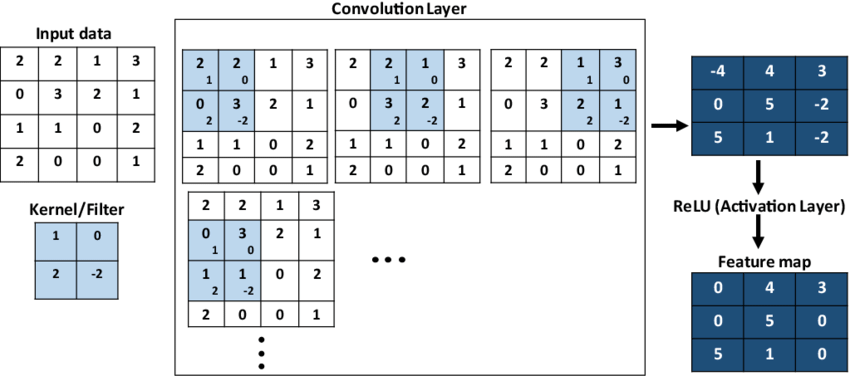
\includegraphics[width=10cm]{archivos/3.Tecnologias/RedesNeuronales/CNN/CNNRELUImage}
                            \caption{https://www.researchgate.net/journal/Transport-in-Porous-Media-1573-1634. Ejemplo de ReLU aplicado a una convolución de dos dimensiones.}
                            \label{CNNRELUImage}
                         \end{figure}

                \end{itemize}

                En el proceso de entrenamiento de las \textit{CNNs} cada uno de los valores de los kernels son optimizados mediante el método \textit{GD}, de tal forma que los pesos de cada capa son actualizados gracias a la derivabilidad de la función de pérdida.\\


                                
                Una \textit{Red Neuronal Convolucional de 1 Dimensión}, o \textit{Convolutional Neural Network 1-Dimensional (CNN-1D)}, es un tipo de red convolucional que utiliza kernels \textit{(filters)} que son aplicados a las imágenes de entrada con el objetivo encontrar ciertas características en ellas.\\

                Las complejidad computacional de las \textit{CNN-1D} es menor que la de las \textit{CNN-2D}, además, estas redes se han demostrado ser más efectivas en distintos campos con respecto a las \textit{CNN-2D}, como en técnicas de análisis de señales. La baja carga computacional de esta arquitectura la hace atractiva para aplicarla en tiempo real en dispositivos con pocos recursos como teléfonos móviles \cite{Conv1D_Survey}.\\


                El resultado de este proceso es la proyección del filtro sobre un espacio dimensional denominado mapa de caracerísticas \textit{(feature maps)}. Este filtro se utiliza para convolucionar los feature maps de la capa anterior \cite{FiltersFeatureMaps} o de la imagen de entrada si se trata de la primera capa de la red.
                

                \begin{figure}[h]
                    \centering
                    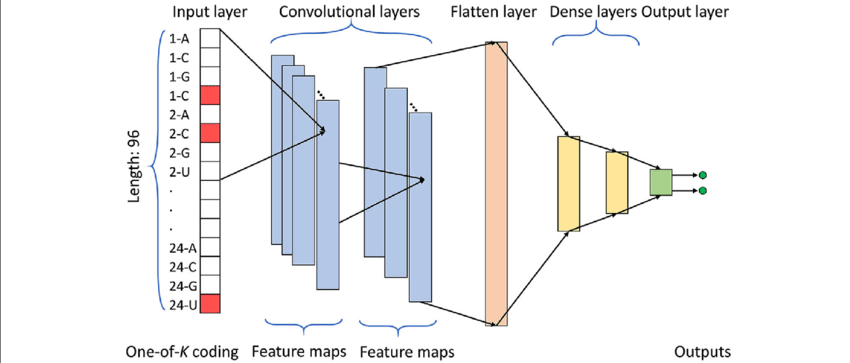
\includegraphics[width=15cm]{archivos/3.Tecnologias/RedesNeuronales/CNN/1D/1CNNArchImage}
                    \caption{https://www.researchgate.net/publication/329201018/figure/fig2/AS:697400008138753@1543284527161/The-architecture-of-our-1D-CNN-model-This-model-consists-of-two-convolutional-layers.png}
                    \label{1CNNArchImage}
                \end{figure}


                Al ser una arquitectura unidimensional, el \textit{kernel} tendrá que tener un tamaño ($1 \times n$).

                \begin{figure}[h]
                    \centering
                    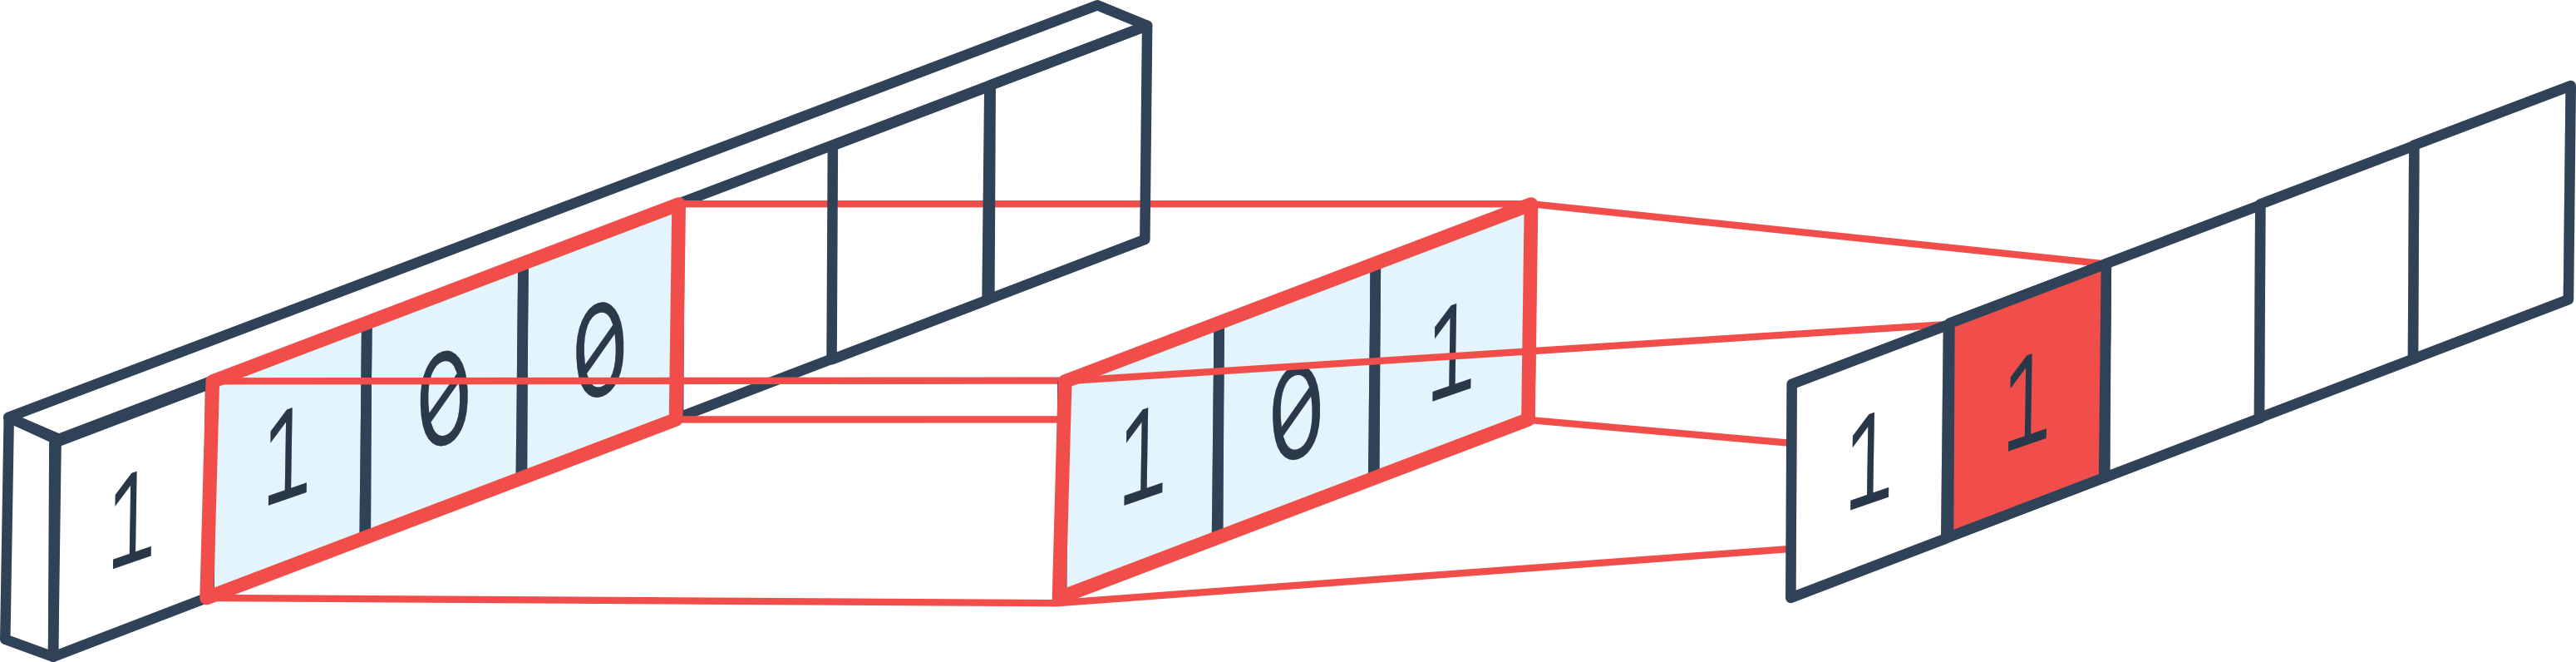
\includegraphics[width=7cm]{archivos/3.Tecnologias/RedesNeuronales/CNN/1D/1DConvolution}
                    \caption{https://peltarion.com/knowledge-center/documentation/modeling-view/build-an-ai-model/blocks/1d-convolution Observamos la entrada de la red (izquierda) a la que se le aplica un kernel (en el centro) que resulta en la convolución de un mapa de características (derecha).}
                    \label{1DConvolutionImage}
                \end{figure}

                    
                Otra de las técnicas convolucionales implementadas en este proyecto son las \textit{Redes Neuronales Convolucionales de 2 Dimensiones}, o \textit{Convolutional Neural Networks 2-Dimensional (CNN-2D)}. Al igual que en el caso de las \textit{CNN-1D}, el filtro se aplica sobre el input de la capa, resultando en \textit{feature maps}, sin embargo, en este caso \textit{kernel} será de bidimensional al ser una convolución de dos dimensiones, por lo que es necesario especificar el tamaño de la matriz que recorrerá la matriz pasada como input a la capa correspondiente.

            \subsection {KNN}

                El algoritmo \textit{K vecinos más próximos}, o \glsentryfull{knn} [\cite{KNN}], es una técnica de aprendizaje supervisado ampliamente utilizada para tareas de clasificación y regresión, es uno de los algoritmos más básicos de \textit{ML} y tiene una gran importancia en el campo de la \textit{Ciencia de Datos} debido a su simplicidad de implementación y a su interpretabilidad.\\

                El algoritmo \textit{KNN} asume que muestras con características parecidas deben pertenecer a la misma clase. O lo que es lo mismo, muestras parecidas deben estar cercanas en el espacio dimensional.\\

                Esta técnica se basa en representar las muestras de un conjunto de datos en base a sus características en un espacio n-dimensional y clasificar la muestra correspondiente como la clase mayoritaria al calcular la distancia de dicha muestra a los $k$ vecinos más próximos. Normalmente la distancia empleada es la \textit{Euclídea}, aunque es posible calcular otras distancias como \textit{Manhattan} o \textit{Chebyshev}.\\
                
                A medida que se incrementan las dimensiones del espacio resulta más costoso computacionalmente calcular distancias entre los puntos.\\


                Por lo tanto, el único parámetro a configurar es el número de vecinos más cercanos que se calculará en base al punto que queramos clasificar, en la figura \ref{KNNImage} se muestra un ejemplo de un problema de clasificacíón aplicando distintos valores al parámetros $k$.

                \begin{figure}[h]
                    \centering
                    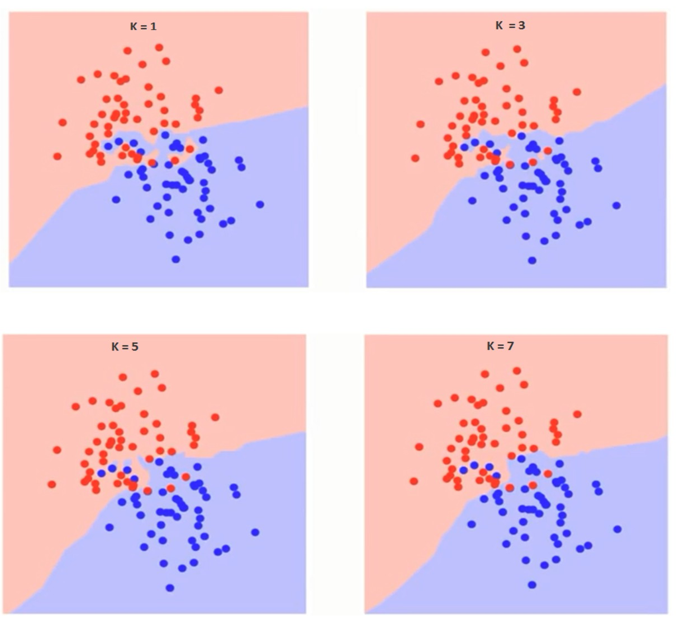
\includegraphics[width=10cm]{archivos/3.Tecnologias/KNN/KNNImage}
                    \caption{https://forum.huawei.com/enterprise/es/data/attachment/forum/202108/20/150033de3l4nyvmcbozh14.png?KNN3.png KNN aplicado con distintos valores de $k$}
                    \label{KNNImage}
                \end{figure}

            

    \section{Especificaciones técnicas}

        En esta sección detallaremos las herramientas que han sido utilizadas para poder realizar este proyecto.


        \subsection{Herramientas utilizadas}
            En primer lugar se ha utilizado de forma intensiva \textit{Python}, que es un lenguaje de programación interpretado de nivel alto multiparadigma. La versión empleada para el desarrollo del proyecto ha sido 3.9.11. \cite{Python}
            
            Las liberías más utilizadas han sido:

            \begin{description}

                \item Pandas: libería que provee de herramientas que permiten el análisis y la manipulación de datos. La versión utilizada para este proyecto es la 1.3.5 \cite{Pandas}.

                \item Tensorflow: libería utilizada para la implementación de redes neuronales permitiendo su ejecución. Este proyecto se basa en la versión 2.8.0 \cite{Tensorflow}.

                \item Sklearn: librería que contiene múltiples modelos predictivos implementados, basado en NumPy, SciPy y Matplotlib. La versión configurada para este proyecto es 1.0.2 \cite{Scikit-Learn}.

                \item XGboost: paquete que contiene la implementación del algoritmo XGBoost, además de múltiples configuraciones como la ejecución en \textit{CPU, GPU y GPU paralelizada}. La importación de esta librería ha sido en base a la versión 1.5.0 \cite{XGBoostLibrary}.

            \end{description}

            Respecto a las herramientas \textit{Software} utilizadas destacan:

            \begin{description}

                \item CUDA: plataforma de computación paralelizada que permite la ejecución de código en \textit{GPU}, esto permite que las redes neuronales puedan entrenarse con mayor rapidez que en \textit{CPU} debido a la velocidad con la que se realizan las operaciones orientadas a datos en las tarjetas gráficas. Se ha utilizado la versión 11.6 \cite{CUDA}.

                \item Anaconda: distribución open-source que ofrece la flexibilidad de mantener varios entornos con distintas configuraciones y versiones de distinas librerías, facilitando además la migración entre equipos. La versión utilizada ha sido la 4.12.0 \cite{Anaconda}.

                \item Jupyter Notebook: entorno interactivo que permite la creación, edición y ejecución de notebooks de forma local y remota. La versión utilizada para el desarrollo de este proyecto ha sido la 6.4.10 \cite{JupyterNotebook}.

                \item Jupyter Lab: interfaz de nueva generación que convive con el entorno Jupyter Notebook, ofrece numerosas funcionalidades como es la navegación entre distintos repositorios dentro de la interfaz. La versión instalada para la realización del proyecto ha sido la 3.3.2 \cite{JupyterLab}.

                \item DiagramsNet: plataforma utilizada para la confección de figuras mostradas en este documento \cite{DiagramsNet}. 

                \item Google Meets: plataforma utilizada para realizar reuniones semanales con el tutor \cite{GoogleMeet}.

            \end{description}

            Como sistema de control de versiones se ha utilizado \cite{Github}, repositorio donde es posible subir versiones evolutivas del proyecto imprescincible en los proyectos de desarrollo \cite{Software}.

        \subsection{Especificaciones del servidor}
            La mayor parte de los experimentos realizados en este trabajo se han ejecutado bajo un servidor con CPU \textit{Dual AMD Rome 7742} (128 cores) y contando con una GPU \textit{DGX NVIDIA A100} de  40 GigaBytes (\textit{GB}).
            